\documentclass[12pt,a4paper]{article}
\usepackage[left=2cm,right=2cm,top=2cm,bottom=2cm]{geometry}


%idioma
\usepackage[utf8]{inputenc}
\usepackage[spanish]{babel}

%hipervinculos
\usepackage{hyperref}

%gráficos
\usepackage{graphicx}
% % % % % % % % % % % % % % % % % % % % % % Fuentes piola


\usepackage{cmbright}


%Bibtex
\usepackage[numbers]{natbib}
%\usepackage[authoryear]{natbib}

\usepackage{amsmath}

%\usepackage[T1]{fontenc}
%\usepackage[scaled]{beramono}
\usepackage{inconsolata}
            
%%%%%%%%%%%%%%%%%%%%%%%%%%%%%%%%%%%%%%%%%%%%%%%%  
%Microtype = estilo más refinado (?)
\usepackage[protrusion=true,expansion=true]{microtype}
%\usepackage{microtype}%Estandar

%%%%%%%%%%%%%%%%%%%%%%%%%%%%%%%%%%%%%%%%%%%%%%%%  
%Gráficos
\usepackage{graphicx}
\usepackage[small]{caption}

%%%%%%%%%%%%%%%%%%%%%%%%%%%%%%%%%%%%%%%%%%%%%%%%  
%Tablas
\usepackage{multirow}
\usepackage{tabularx} %tablas con mucho texto
\usepackage{booktabs}

%Listings para código fuente
\usepackage{listings}
\lstset{
basicstyle=\small\ttfamily,
%numbers=left,
%numberstyle=\tiny,
%frame=tb,
resetmargins=true,
%columns=fullflexible,
showstringspaces=false,
%numberstyle=\tiny\sffamily,
%stepnumber=10,
}


%%%%%%%%%%%%%%%%%%%%%%%%%%%%%%%%%%%%%%%%%%%%%%%%  
% Cabecera y pie de página
\usepackage{fancyhdr}

\pagestyle{fancy}
\fancyhf{} %Limpia las cabeceras
\renewcommand{\headrulewidth}{0pt}
\fancyhead[L]{\footnotesize\bfseries  [75.06] Organización de Datos}
%\fancyhead[C]{}
\fancyhead[R]{\footnotesize\bfseries  Diseño TP - Grupo 20}

\fancyfoot[L]{}
\fancyfoot[C]{\thepage}
\fancyfoot[R]{}
\renewcommand{\headrulewidth}{0.4pt}
\renewcommand{\footrulewidth}{0.6pt}

%%%%%%%%%%%%%%%%%%%%%%%%%%%%%%%%%%%%%%%%%%%%%%%%  
%Contador de secciones empieza en 0
%\setcounter{section}{-1}

%%%%%%%%%%%%%%%%%%%%%%%%%%%%%%%%%%%%%%%%%%%%%%%%  
%Fin declaraciones

\begin{document}
\bibliographystyle{plainnat}


\begin{titlepage}

\begin{flushleft}

\includegraphics[width=0.4\textwidth]{./Images/logoFiubaCompleto}
\end{flushleft}

\begin{center}
\sffamily
\bfseries
\large

\vspace*{\fill}

Organización de Datos (75.06)

%\vspace*{\fill}

Curso 01 - L. Argerich

\vspace*{\fill}

Trabajo Práctico

\resizebox{0.6\linewidth}{!}{Indexador de Textos}

1ro/2013

\vspace*{\fill}

\begin{table}[!h]
\normalfont
\centering
\large

\begin{tabular}{l l}
\toprule
Amarillo, Emilio & 88343 \\
Arias, Damián & 89952\\
Gattei, Ignacio & 91664\\
Tarsia, Guido & 91456\\
\bottomrule
\end{tabular}
\end{table}

\vspace*{\fill}

\end{center}
\end{titlepage}

\tableofcontents
\newpage

\section{Introducción}

El objetivo de este Trabajo Práctico es realizar un programa que permita buscar frases en un conjunto de documentos (la colección).

Para ello, luego de investigar sobre el tema, concluimos que la estructura más popular para este tipo de aplicación es el índice invertido, que consiste de dos grandes componentes: el vocabulario de términos (por ejemplo, de palabras) de la colección, y una lista invertida, la cual es una estructura que contiene información sobre la ocurrencia (o posición) del término.

Para la búsqueda de frases en índices invertidos se han propuesto diferentes enfoques. La primera estrategia, propuesta en \citet{Williams99what'snext?} (\citeyear{Williams99what'snext?}) sería guardar palabras contiguas, en lo que se llama un índice de próxima palabra (nextword index). En la frase <<hoy hace calor>> se guardarían <<hoy hace>> y <<hace calor>> acompañado del documento en donde aparecen. Este enfoque podría utilizar hasta aproximadamente el doble de espacio en disco que la colección, porque se guardan todas las palabras de los documentos en dúos que pueden tener muy poca repetición. Se crean índices, aunque de tamaño considerable, de rápido accionar para encontrar frases.

Otra estrategia, la que utilizaremos, es almacenar la posición de cada término en cada documento de forma ordenada, así pueden utilizarse distintos algoritmos de compresión. Para buscar una frase, primero se buscan todas las palabras que contiene y se obtienen las listas invertidas para cada una, extrayendo las posiciones y documentos en donde aparecen las mismas. Luego, aplicando un algoritmo de intersección, se filtran los documentos en donde las palabras efectivamente existen en el orden deseado.

Una última estrategia, bastante más sofisticada, sería la presentada por \citet{Williams:2004:FPQ:1028099.1028102} (\citeyear{Williams:2004:FPQ:1028099.1028102}) en donde se hace una combinación de las anteriores (un índice invertido con las palabras menos comunes y un indice de próxima palabra con los dúos más comunes) pero agregando un índice con las frases más comunes. Esta aproximación acelera un 400 \% el tiempo de búsqueda sobre nuestra propuesta, pero ocupa el doble de espacio en disco, según el mismo artículo. Como priorizamos espacio antes que tiempo, la idea es descartada.




\section{Definiciones básicas}

Para diagramar el trabajo primero estableceremos las siguientes definiciones básicas:
\begin{itemize}

%\item Consulta (q): es una ni idea que poner

\item Documento: conjunto de datos en formato estándar de texto (Unicode).

\item Carpeta a indexar: es la que se le pasa al programa creado para que procese todos sus documentos, y permita hacer consultas sobre su contenido

\item Colección: conjunto de todos los documentos que aparecen en la carpeta a indexar.

\item Diccionario: conjunto de todos los términos.

\end{itemize}


%\subsection{Término (\textit{\textnormal{T}})}
\subsection{Término (\textnormal{\itshape T})}

 
Se considera término \textit{T} a todo conjunto de caracteres alfanumérico sumados al apóstrofo (o comilla simple: ' ). Cada término es, o bien, una cantidad numérica desde 1 (una) hasta una cantidad no definida de cifras, o bien palabras tanto simples como compuestas. Se desarrolla sobre este tema en la Sección \ref{sec:parser}.


\subsection{docID (\textnormal{\itshape D})}
\noindent (\textit{document identification} = identificador de documento)

Este es un número asignado unívocamente a cada documento de la carpeta a indexar. Para hacer este proceso, se listan recursivamente todos los documentos (que se suponen \textit{indexables}, es decir, de texto plano) y se los ordena (el criterio será develado más adelante). Este orden otorga el docID de cada documento, que comienzan desde el 1 (uno).


\subsection{d-gap}
\noindent(\textit{document-gap} = distancia entre documentos)

Considerando una lista de docIDs en orden ascendente, se puede almacenar la misma con el primer elemento seguido de las diferencias entre los elementos siguientes, los \textit{d-gaps}. Se utiliza la definición dada en \citet[p.~115]{WittenMoffatBell99}.

Por ejemplo $\langle 1, 2, 4 , 5 , 8 \rangle$ se puede transformar en $\langle 1, 1, 2 , 1 , 3 \rangle$.



%\citeauthor[p.~115]{WittenMoffatBell99}.

%\subsection{Frecuencia absoluta (\textnormal{\itshape F \texorpdfstring{\textsubscript{F}})}}
\subsection{Frecuencia absoluta (\texorpdfstring{$F_{T}$}{FF})}

Cantidad de veces que aparece un término \textit{T} en toda la colección.


%\subsection{Frecuencia relativa (\textnormal{\itshape f \texorpdfstring\textsubscript{D,T}})}
\subsection{Frecuencia relativa (\texorpdfstring{$F_{D,T}$}{FFD})}

Cantidad de veces que aparece un término \textit{T} en un documento \textit{D}.

\subsection{Lista de posiciones}

También llamada lista de ocurrencias. Es aquella que almacena las posiciones $p_i$ en un documento \textit{D} en donde aparece el término \textit{T}. Una posición en un documento corresponde a la cantidad de términos hasta el término en consideración, empezando por el 1.
%\begin{center}
%    \includegraphics[scale=0.8]{./images/graf9}
%    
\includegraphics[width=0.4\textwidth]{./images/logoFiubaCompleto}
%\end{center}

\section{Generación de términos}\label{sec:parser}
 
Todos los términos estarán compuestos de una única palabra y se guardarán en el Diccionario con letras minúsculas. Se tomaron decisiones basándonos en las siguientes directivas.


\subsection{No se guardarán términos de más de una palabra}

Aunque los indices tipo Nextword (próxima palabra) son capaces de otorgar velocidades de acceso superiores a los índices invertidos tradicionales, ocupan en promedio un 60 \% del espacio de la colección, según mencionan \citet{Williams99what'snext?} (\citeyear{Williams99what'snext?}). 

Para este Trabajo Práctico, se construirá un índice preparado para buscar frases, pero a través de sus posiciones. Esto quiere decir que se tendrán en cuenta la separación entre palabras dentro de un documento. Por ejemplo un sustantivo propio de más de una palabra como <<San Francisco>> se separará en dos términos <<San>> y <<Francisco>>. Al hacer la consulta el programa calculará la distancia entre las dos palabras: (<<San>>, posición $i$) y (<<Francisco>>, posición $i+1$), con las cuales se podrá intersecar con las listas invertidas de cada una y filtrar los documentos en donde en aparecen juntas en las posición requerida.


\subsection{Se guardarán todos los términos en letra minúscula}
En un texto, puede haber palabras que contengan mayúsculas en los siguientes casos:

%comiencen con una letra mayúscula solo en 2 casos:

\begin{itemize}
\item Mayúscula al comenzar la palabra: porque es un sustantivo propio
\item Mayúscula al comenzar la palabra: porque está precedida por un punto <<.>>
\item Mayúscula en medio de la palabra: porque es un código o abreviatura (<<IQJ653>>, <<PhD>>)
\end{itemize}

Esto sería un problema si quisiéramos guardar términos de más de una palabra como en el ejemplo anterior ya que se complicaría enormemente para identificar <<San Francisco>> en el siguiente escenario: <<… buenos momentos. San Francisco es …>>. No hay forma de saber si <<San>> empieza con mayúscula porque es un sustantivo propio o porque está al lado de un punto. Por suerte, esto no será un problema, ya que se guardará todo en minúsculas.

Que todo se guarde en minúsculas, también ayuda en la búsqueda, ya que el usuario del programa podría escribir de forma incorrecta sin poner las mayúsculas e igualmente encontrar lo que busca.

 
 
\subsection{Casos particulares de signos de puntuación}
 
\begin{itemize}

\item Guiones: si se encuentra un guion (medio o bajo) se toma como si fuese un espacio. Si el guion está dividiendo 2 palabras, se guarda cada palabra por separado como un término. También se reemplazan por espacios las ‘@’ y los ‘/’.

\item Apóstrofo (o comilla simple): por estar los textos de la colección en idioma inglés, conviene contemplar algunos casos del uso del apóstrofo y como se los tratará, a través de los siguientes ejemplos:
\begin{itemize}

\item  <<Grey’s Anatomy>>: en este caso, se guardarán los términos <<grey's>> y <<anatomy>> por separado.
\item  <<Isn’t it?>>: se guardará <<isn't>> y <<it>>.
\item  <<Baba O’Riley>>:  se guardará <<baba>> y <<o'riley>>.
\item  Caracteres que se ignoran: todos los caracteres que no son alfanuméricos y <<encierran>> conjuntos de palabras como son \texttt{¿?¡!()[]{}}, comillas dobles, acentos graves y agudos.
% ’’. 
También se ignoran \texttt{.:,;~ * \^{} +- \$ \#} .

\end{itemize}

\end{itemize}

\subsection{Números}

Los números se guardarán como términos comunes y silvestres. Por ejemplo:

\begin{itemize}
\item <<1000>> $\Longrightarrow$ <<1000>>
%\item <<1.000>> $\Longrightarrow$ <<1.000>>
\item <<03/04/2004>> $\Longrightarrow$ <<03>>, <<04>> y <<2004>>
\end{itemize}


\section{Construcción del índice: primera parte}

Se mostrará la creación del índice a través de un ejemplo: se quiere indexar la carpeta <<vainilla/>> la cual contiene 3 documentos.

\begin{figure}[!h]
\centering
    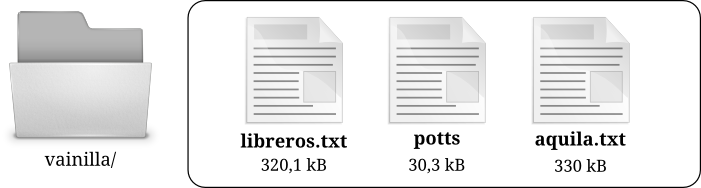
\includegraphics[scale=0.9]{./Images/vainillaDir.png}
\caption{Ejemplo de directorio de trabajo}
\label{fig:directorioTrabajo}
\end{figure}


\subsection{Lectura del directorio y asignaciones de docIDs}

Luego de verificar que el directorio a indexar existe, se leen los nombres de \textbf{todos} los documentos del mismo (consideramos que el directorio es de \textit{buena fe}), incluyendo los contenidos en carpetas interiores. Se ordenan los nombres alfabéticamente y se les asigna un docID correlativamente con el orden, es decir, el archivo que queda con el nombre en primera posición tiene el docID más bajo, el cual en el esquema propuesto por nosotros, es 1 (uno). Así se sigue hasta el último documento.

\subsection{Extracción de términos y creación del índice en memoria}

\begin{figure}[!h]
\centering
    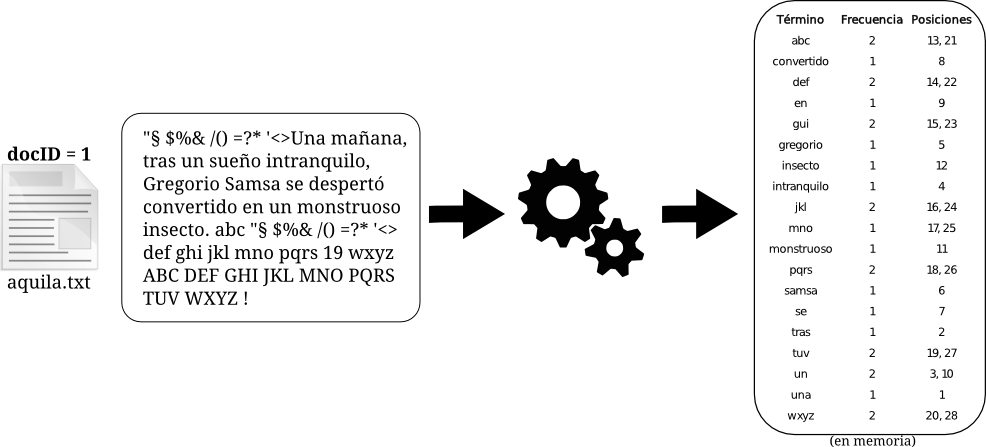
\includegraphics[scale=0.9]{./Images/parseoYMem.png}
\caption{Un archivo procesado y cargados sus términos en memoria}
\label{fig:parseoymem}
\end{figure}

Como mencionamos en la Sección \ref{sec:parser} cada término es una palabra o cifra numérica. El programa crea listados en memoria principal con la siguiente información: para un término $T_i$ se almacena que aparece en el documento con docID $D_1$ en las posiciones $p_1, p_2, p_3 \ldots p_m$, y listados equivalentes para los demás documentos. La estructura de estos listados es:

\[
\left\lbrace T_i ;
    \left( D_1 , 
        \left\langle
            p_1, p_2, p_3 \ldots p_m 
        \right\rangle  
    \right)
    ;
    \left( D_2 , 
        \left\langle
            p_1, \ldots p_f
        \right\rangle  
    \right) 
    ;
    \ldots
    ;
    \left( D_j , 
        \left\langle
            \dots
        \right\rangle  
    \right) 
\right\rbrace 
\]

Este procedimiento (generar términos y llevarlos a memorias principal) se hace constantemente hasta que ocurra uno de los siguientes hechos:

\begin{enumerate}
\item Se terminen de procesar todos los documentos
\item Se ocupe toda la memoria dedicada para el programa (se requerirán 512 MB de RAM dedicados, es decir, una PC con al menos 1 GB en total). En tal caso se crearán archivos temporales, se vaciará la memoria y se vuelve al paso 1.
\end{enumerate}


\subsection{Creación de archivos temporales}

La primera vez que ocurra uno de estos dos momentos se creará un directorio temporal <<vainillatemp/>> que irá guardando archivos temporales con la información tal cual aparece en memoria. Sucesivas bajadas de memoria a disco, generarán archivos temporales de nombre incremental.

\begin{figure}[!h]
\centering
    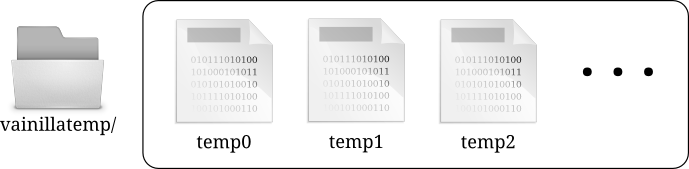
\includegraphics[scale=0.9]{./Images/tempDirEstr.png}
\caption{Un directorio temporal con archivos temporales}
\label{fig:tempdir}
\end{figure}


Cada archivo temporal contiene información suficiente para armar un índice por si mismo, ya que almacena para los documentos procesados, los términos, docIDs, frecuencias relativas y lista de posiciones como se muestra en la Figura \ref{fig:tempfile}.


\begin{figure}[!h]
\centering
    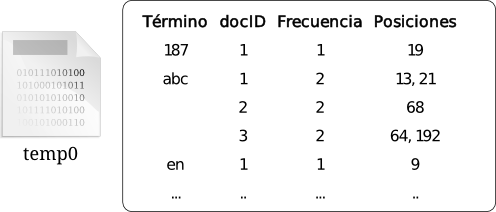
\includegraphics[scale=0.9]{./Images/tempFileEstr.png}
\caption{Datos almacenados en un archivo temporal}
\label{fig:tempfile}
\end{figure}


%\begin{figure}[here]
%\includegraphics[width=0.9\textwidth]{images/JobInformationDialog.jpg}
%\caption{A prototype of the Job Information dialog}
%\label{fig:jobInformationDialog}
%\end{figure}

\section{Construcción del índice: segunda parte}

Se continuará utilizando el ejemplo.

\subsection{Merge-Based Inversion}

Es inevitable citar a \citet[p. ~14]{Zobel06invertedfiles} (\citeyear{Zobel06invertedfiles}) y \citet[p.~238]{WittenMoffatBell99} \citeyear{WittenMoffatBell99}, en donde encontramos

Merge-based index construction is practical for collections of all sizes. In particular,
it scales well and operates effectively in as little as 100MB of memory. In addition, disk
space overheads can be restricted to a small fraction of the final index; only one parsing
pass is required over the data; and the method extends naturally to phrase indexing.
Finally, the compression techniques described in Section 8 can further reduce the cost
of index construction by reducing the number of runs required.


%\begin{figure}[!h]
%\centering
%    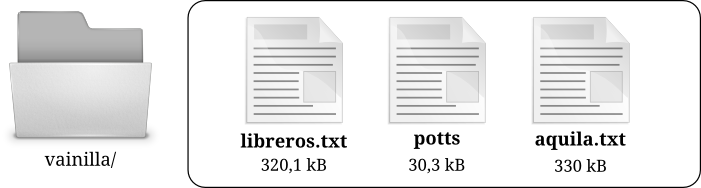
\includegraphics[scale=0.9]{./Images/vainillaDir.png}
%\caption{Ejemplo de directorio de trabajo}
%\label{fig:directorioTrabajo}
%\end{figure}




\section{Métodos de compresión}

Para elegir métodos de compresión para listas de enteros se ha consultado:

\begin{itemize}

\item \citet{Trotman:2003}, (\citeyear{Trotman:2003}): se analizan los métodos Variable Byte (<<vByte>>), Delta, Gamma y Golomb, extrayendo la conclusión que la tasa de compresión es exactamente inversa al listado de los nombres. Golomb obtiene un 50 \% mayor compresión que vByte, mientras que este descomprime 7 veces más rápido que Golomb. Los otros métodos se ubican en el medio de estas cifras, sin alejarse demasiado de Golomb.

\item \citet{Anh:2005}, (\citeyear{Anh:2005}): propone 3 algoritmos de rápida descompresión <<Simple-9>> (S9), <<Relative-10>> y <<Carryover-12>> y los compara a Golomb. Las conclusiones son que Golomb provee entre un 10 \% y un 25\% más compresión que los propuestos, mientras que es hasta un 200 \% más lento para recuperar información.

\item \citet{Zhang:2008}, (\citeyear{Zhang:2008}): analizan S9, vByte, PFor y Rice, y se extraen las conclusiones que Rice es el que mayor tasa de compresión ofrece, muy poco por encima de la compresión óptima, el método de PFor es alrededor de 4 veces rápido al descomprimir apenas ocupando un pequeño porcentaje de almacenamiento de más comparado a Rice.

\item \citet[p.~210]{Buettcher2010}, (\citeyear{Buettcher2010}): analizan Gamma, Delta, Golomb, Rice, vByte y S9. Como es el único que tiene a Golomb y Rice juntos, se extraen conclusiones importantes de aquí. Se puede observar Golomb tiene una ventaja insignificante en cuanto a tasa de compresión, pero es tiene una desventaja importante en cuanto a velocidad de descompresión. En datos duros, es como ganar un 2 \% de espacio, pero perder un 30 \% más de tiempo en descomprimir (la compresión demora lo mismo en ambos).



\end{itemize}

\subsection{Rice coding}

El primero elegido es Rice coding. Conocido hoy en día como un caso particular de Golomb coding, es uno de los métodos más antiguos de compresión, data del año 1979. Se trata de que un entero $n$ es codificado en 2 partes: un cociente $\lfloor \frac{n}{2^b} \rfloor$ y un resto 
$r = n \text{ mod } 2^b$. El cociente es almacenado en forma unaria utilizando $q+1$ bits, mientras que el resto es almacenado en formato binario usando $b$ bits. 


%En nuestra implementación, el parámetro $b$ es elegido por bloque, entonces $2^b$ es cercano al valor medio del bloque.

La ventaja principal de este método es que tiene muy buena tasa de compresión. Sin embargo es en general un método lento en términos de velocidad de compresión y descompresión, siendo la causa principal que este método necesita manipular el código unario un bit a la vez, tanto en compresión, como en descompresión. Esto es muy demandante para el CPU, pero, por otro lado, como $b$ es potencia de 2, la compresión y descompresión se hacen lo más eficientemente posible, necesitando operaciones bit a bit, como shifts y máscaras. 

Golomb comprime con un $b= 0.69 \times Promedio$ (promedio de todos los números de la lista a comprimir), y se necesitarán múltiplicaciones y divisiones que enlentecen los procesos de compresión y descompresión. En teoría alcanza mejor tasa de compresión que nuestro elegido Rice, pero en la práctica la diferencia es muy pequeña \cite{Zhang:2008}, \cite{Buettcher2010}.

%En nuestra implementación codificaremos una lista de $n$ enteros (con $n$ múltiplo de 32) a la vez. Primero se guardarán todas las partes binarias, utilizando $b$ bits, o sea que en total se ocuparán $n \dot b$ bits para todos. Luego se almacenarán las pares unarias.

\subsection{Frame of reference (FOR)}

(\noindent \textit{Adaptado de \citet[p.~5]{Delbru10adaptiveframe} (\citeyear{Delbru10adaptiveframe})})
\\

El método FOR determina el rango de posibles valores en una lista, llamada \textit\textbf{<<marco de referencia>>} y mapea cada valor adentro de este rango guardando suficientes bits para que los valores puedan ser distinguibles. 

Por ejemplo, se tiene el siguiente listado (medianamente ordenado y con repetición): 
\[\left< 107,108,110,115,120,125,132,132,131,135 \right> \]

Si utilizáramos 8 bits para almacenar los cada uno de los 10 números, ocuparíamos 80 bits. En cambio, utilizando el punto de vista FOR, veríamos que el rango de número va de 107 a 135, por lo que podríamos restar 107 a todos los números de la secuencia, quedando $\left< 0, 1, 3, 8, 13, 18, 25, 25, 24, 28 \right>$. Ahora cada diferencia puede codificarse con a lo sumo 5 bits. Por supuesto que debe guardarse el mínimo valor utilizando 8 bits, y también indicar con 3 bits más el hecho que solo son 5 bits por valor. En total se ocuparon $(8+3+9*5=45)$ bits, ahorrando un 44 \% con respecto a la opción sin compresión.

Hay un beneficio fundamental de este método relacionado con el guardado de grandes enteros: si quisiéramos el número 25312 y encontramos que el valor mínimo de la lista comprimida es 107 y se usan 5 bits para guardar los elementos, sabremos de entrada que esa lista no tiene el elemento que buscamos.

Dado un marco de referencia $[0, max]$, FOR necesita $\lceil \log_2(max+1) \rceil$ bits, llamados \textit{bits del marco}, para comprimir cada entero en el listado. 

La principal desventaja de FOR es que es sensible a valores atípicos en un grupo de valores. Por ejemplo, si un listado de 1024 enteros contiene 1023 números inferiores a 16 y un solo valor superior a 128, los \textit{bits del marco} serán $\lceil \log_2(128+1) \rceil = 8$, desperdiciando 4 bits por cada otro valor.

Sin embargo la compresión la compresión y descompresión se pueden hacer muy rápidamente, utilizando operaciones de muy poco coste para el CPU. Se utilizan para ello algoritmos con operaciones lógicas bit a bit como AND o SHIFT, sin estructuras de selección que demoran más tiempo en ejecutarse. Esta es la clave de los algoritmos FOR. Se ve un ejemplo en la Tabla \ref{tabla:FOR}.






%However, compression and decompression is done very efficiently using highly-optimised routines [18] which avoid branching conditions. Each routine is loop-unrolled to encode or decode m values using shift and mask operations only. Listing 1 and 2 show the routines to encode or decode 8 integers with a bit frame of 3. There is a compression and decompression routines for each bit frame.

Dado un listado de $n$ enteros, FOR determina el marco de referencia y codifica el listado a través de pequeñas iteraciones de $m$ enteros usando la misma rutina de compresión en cada iteración. Por cuestiones de rendimiento, $m$ es generalmente elegido múltiplo de 8 para que coincida con la frontera de los bytes.


%In our implementation, FOR relies on routines to encode and decode 32 values at a time.

%La selección de la rutina apropiada para un marco de bits es hecha por una tabla de búsqueda. Al momento de compresión se pasa solo una vez por la lista a comprimir para determinar el marco de bits. Luego se selecciona la rutina asociada al mismo a través de la tabla de búsqueda. Finalmente el marco de bits es almacenado

%The selection of the appropriate routine for a given bit frame is done using a precomputed lookup table. The compression step performs one pass only over the block to determine the bit frame. Then, it selects the routine associated to the bit frame using the lookup table. Finally, the bit frame is stored using one byte in the block header and the compression routine is executed to encode the block. During decompression, FOR reads the bit frame, performs one table lookup to select the decompression routine and executes iteratively the routine over the compressed block.




\begin{table}[!h]
\centering
\small
\begin{tabular}{l l}
\toprule
\begin{lstlisting}[language=C]
compress3 (int[] i, byte[] b)
{b[0] = (i[0] & 7) 
| ((i[1] & 7) << 3) 
| ((i[2] & 3) << 6); 
b[1] = ((i[2] >> 2) & 1) 
| ((i[3] & 7) << 1) 
| ((i[4] & 7) << 4) 
| ((i[5] & 1) << 7); 
b[2] = ((i[5] >> 1) & 3) 
| ((i[6] & 7) << 2) 
| ((i[7] & 7) << 5);}
\end{lstlisting}
&
\begin{lstlisting}[language=C]
decompress3(byte[] b, int[] i)
{i[0] = (b[0] & 7);
i[1] = (b[0] >> 3) & 7;
i[2] = ((b[1] & 1) << 2)
| (b[0] >> 6);
i[3] = (b[1] >> 1) & 7;
i[4] = (b[1] >> 4) & 7;
i[5] = ((b[2] & 3) << 1)
| (b[1] >> 7);
i[6] = (b[2] >> 2) & 7;
i[7] = (b[2] >> 5) & 7;}
\end{lstlisting}\\
\midrule
Rutina de compresión que codifica 8
&
Rutina de descompresión que decodifica 8 \\
enteros usando 3 bits cada uno 
&
enteros representados por 3 bits cada uno\\
\bottomrule
\end{tabular}
\caption{Compresión y descompresión FOR}\label{tabla:FOR}
\end{table}


En el caso de listas \textit{delta} (como la de \textit{d-gaps} presentada anteriormente), como la distribución de probabilidad generada tomando las diferencias tiende a ser monótonamente decreciente, una práctica común es elegir como marco de referencia $[0, max]$, en donde $max$ es mayor valor entre los \textit{deltas}. 


\subsection{PFOR (\textit{patched-FOR})}

(\noindent \citeauthor{Zukowski:2006}, \citeyear{Zukowski:2006})
\\

El segundo elegido. PFOR es una sencilla modificación al método FOR, con la cual se atenúa el problema con valores atípicos mencionado anteriormente (aquí denominados \textit{excepciones}). Primero se determina el valor $b$ para el cual la mayoría (digamos, el 90 \%) de la lista de enteros a comprimir son menores a $2^b$. Entonces el listado comprimido se guarda en 2 partes: en la primera entran todos los enteros menores a $2^b$ en $b$ bits cada uno, y en la segunda se guardan las \textit{excepciones}, con 8, 16 o 32 bits cada una, dependiendo la excepción más grande.

Al igual que FOR es rápido en la compresión y descompresión, salvo por un pequeño número de elementos, las excepciones. Pero tiene mayor tasa de compresión al no desperdiciar tantos bits en listados en donde los valores son en promedio uniformes salvo por algunos particulares.

Este método, modificado para \textit{listas delta}, es llamado en la bibliografía, como en \cite{Zhang:2008} y \cite{Zukowski:2006}, \textbf{PFOR-Delta}.


\subsection{LZW}

Como se verá más adelante, nuestra propuesta para resolver el TP necesita un archivo con palabras guardadas, el Diccionario. 

Para comprimir dicho archivo utilizaremos unos de los métodos clásicos y más simples de compresión, el LZW. Básicamente lo que hace este método es leer una secuencia de símbolos, agruparlos en cadenas de caracteres y convertir las mismas en códigos. Como los códigos ocupan menos lugar que las cadenas de caracteres, se obtiene compresión.

No se hace ningún análisis del texto. En su lugar, solamente agrega cada nueva cadena de caracteres que encuentra a una tabla de que contiene todas las anteriores.

LZW es un algoritmo <<voraz>> (\textit{greedy}) porque trata de encontrar la cadena de caracteres más larga posible para la cual tiene código asignado.


%\begin{lstlisting}[caption=Algoritmo LZW: compresión, label=listing:lzw]
%    STRING = get input character
%    WHILE there are still input characters DO
%        CHARACTER = get input character
%        IF STRING+CHARACTER is in the string table then
%            STRING = STRING+character
%        ELSE
%            output the code for STRING
%            add STRING+CHARACTER to the string table
%            STRING = CHARACTER
%        END of IF
%    END of WHILE
%    output the code for STRING
%\end{lstlisting}
%
%\begin{lstlisting}[caption=Algoritmo LZW: descompresión, label=listing:deslzw]
%Read OLD_CODE
%output OLD_CODE
%WHILE there are still input characters DO
%	Read NEW_CODE
%	STRING = get translation of NEW_CODE
%	output STRING
%	CHARACTER = first character in STRING
%	add OLD_CODE + CHARACTER to the translation table
%	OLD_CODE = NEW_CODE
%END of WHILE
%\end{lstlisting}

\section{Estructuras utilizadas en los archivos}

Como mencionamos en la Sección \ref{sec:indice2}, para guardar toda la información referente a la colección de documentos, utilizaremos 4 archivos.

Combinando los enfoques de \citet{Zhang:2008}, (\citeyear{Zhang:2008}) y de \citet[p.~107]{Buettcher2010}, (\citeyear{Buettcher2010}), llegamos a las estructuras de archivos que describiremos.


\subsection{Los archivos flacos}

Estos archivos solamente almacenan un tipo de dato muy específico:

\begin{itemize}

\item \textbf{*.dic}: aquí se guardan todas los términos que se encontraron en la colección, una larga cadena con los mismos, separados con barra <</>> o espacio. Se los comprime con LZW, en bloques o bien se testeará con todo el archivo. 

\item \textbf{*.frq}: correspondientemente a cada término existe una frecuencia absoluta asociada, que se guarda en este archivo. Lógicamente son enteros sin orden distribuidos aleatoriamente. Se utilizará Rice coding, que es que mejor comprime, para conjuntos de frecuencias. Este archivo tiene la finalidad de ayudar a hacer las búsquedas más rápidas, ya que se irá filtrando por la palabra menos frecuente.

\item \textbf{*.ofs}: además se necesita guardar el offset (distancia) que existe para cierto término en el índice invertido. Como son enteros crecientes que se van a cargar en memoria principal, se utilizan deltas. Hay 2 opciones, o se comprime aplicando Rice coding o PFOR-Delta, separando en conjuntos de offsets, o se deja sin comprimir. Analizaremos si vale la pena el espacio se pierde con la última opción.


\begin{figure}[!h]
\centering
    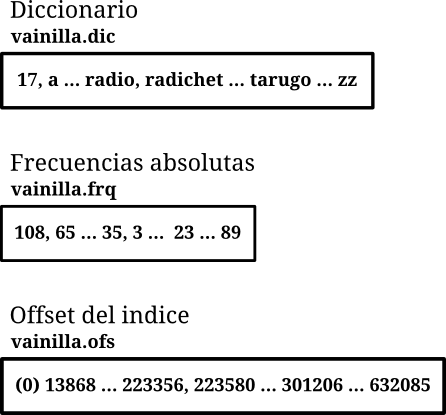
\includegraphics[scale=0.9]{./Images/estructura_2.png}
\caption{Los archivos flacos}
\label{fig:flacos}
\end{figure}



\end{itemize}

\subsection{El índice invertido}

El llamado índice invertido de posiciones sigue con total naturalidad lo propuesto por \cite{Zhang:2008}, pero sin bloques de tamaño de fijo, si no variables (en la frontera de los bytes).

La estructura general de nuestro índice invertido se muestra en la Figura \ref{fig:indice}. Se crean particiones en el archivo llamadas \textit{bloques}, de tamaño variable. 

\begin{figure}[h]
\centering
    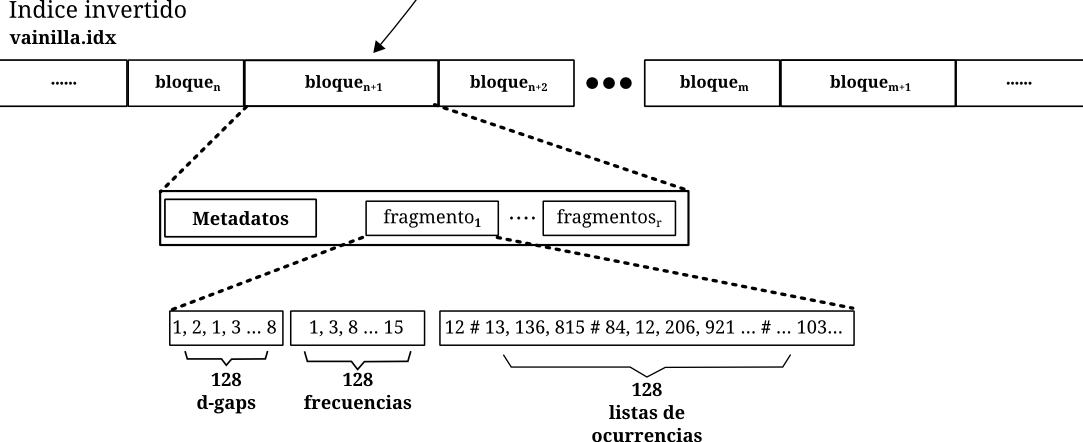
\includegraphics[scale=0.9]{./Images/estructura_1.png}
\caption{Estructura del índice invertido}
\label{fig:indice}
\end{figure}


Definimos un <<posteo>> como el conjunto de un docID, frecuencia relativa y lista de posiciones para un término (lógicamente, en un documento).

\paragraph{Un bloque}

\begin{itemize}

\item Guarda información correspondiente a un término de la colección.

\item Posee un gran número de listas invertidas correspondientes a las posiciones del término en consideración. Siguiendo con la referencia, dividimos estas listas en fragmentos con 128 posteos cada una. Este número podría cambiar para hacer más rápida la búsqueda en colecciones chicas o más grandes, pero siempre será múltiplo de 32.

\item Contiene metadatos (datos adicionales) con información de cuántos fragmentos posee y dónde comienzan (offset desde el primer fragmento), y a continuación los fragmentos. Esto se hace porque, como la estructura de datos permite decodificar los docIDs primero que lo demás, se quiere ser capaz de saltar al siguiente fragmento sin pasar por todos los datos comprimidos. No se decidió si comprimir los metadatos aún.

\end{itemize}

\paragraph{Un fragmento}

\begin{itemize}

\item Es una unidad básica para descomprimir datos en el índice invertido. Cada fragmento se puede descomprimir muy rápidamente.

\item Contiene 128 posteos almacenados como: 128 docIDs (almacenados como \textit{d-gaps}), luego 128 frecuencias relativas correspondientes y al final 128 listas de ocurrencias (guardadas como \textit{gaps} para cada docID). Los métodos de compresión serán, respectivamente, PFOR-Delta, Rice coding y PFOR-Delta nuevamente (a prueba, si no Rice coding).

\item Se lo puede <<saltar>> si el docID que buscamos no se encuentra, por ello este listado se comprime con PFOR-Delta (que guarda la el rango  máximo y el primer docID).

\end{itemize}


\section{Haciendo consultas}

En esta sección se ilustrará cómo funciona el algoritmo que utiliza el programa al momento de resolver una consulta.

% Asumo que levantamos la tabla en memoria cada vez que se realiza una consulta. No es lo ideal, pero es lo que pide el enunciado.
\subsection{Puesta en marcha}

\begin{figure}[!ht]
\centering
    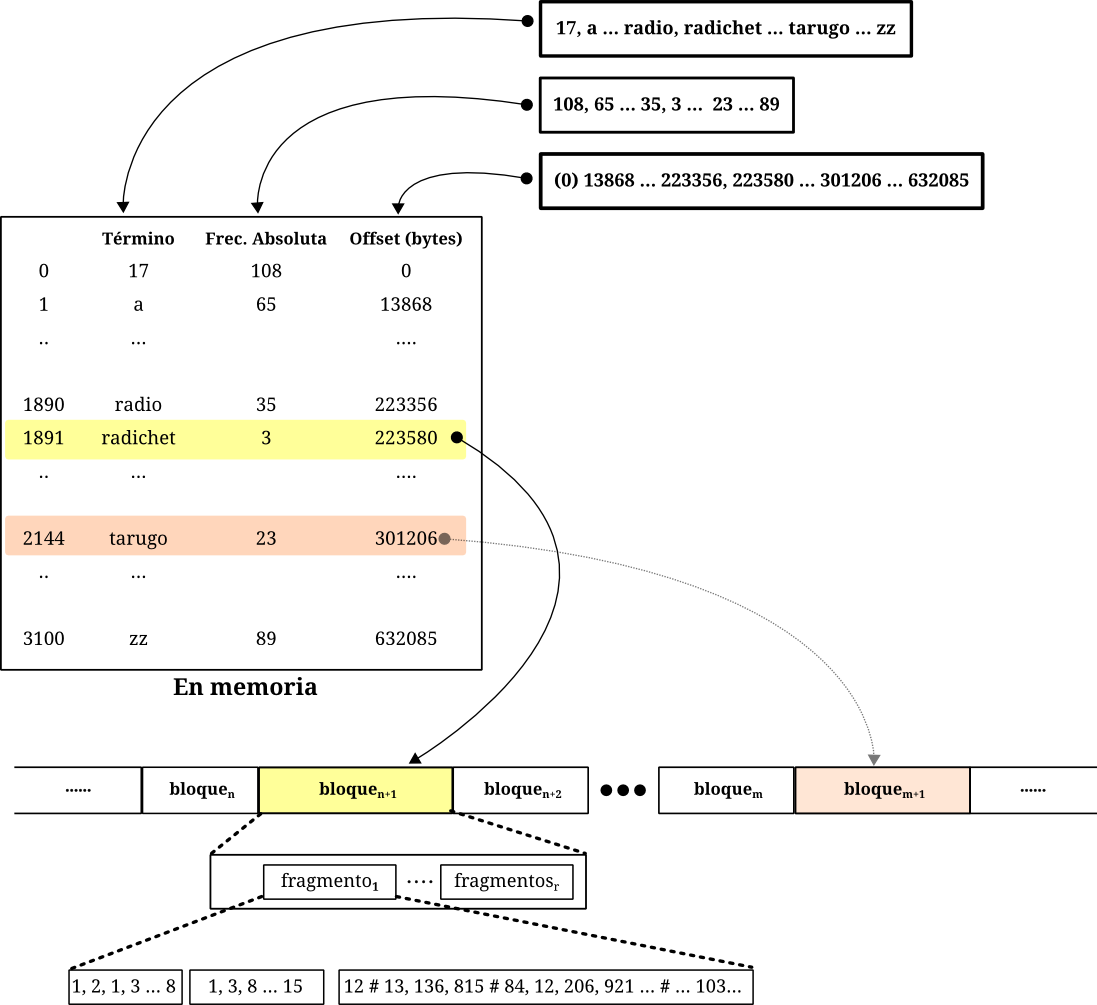
\includegraphics[scale=0.8]{./Images/consulta1.png}
\caption{Armado en memoria de la tabla de términos y búsqueda en el índice invertido}
\label{fig:consulta1}
\end{figure}


Ni bien se ejecuta el programa, éste se prepara para resolver la consulta armando para ello una tabla en memoria. Esta tabla se compondrá de tres columnas: Término, Frecuencia Absoluta y Offset.

Cada columna se extrae descomprimiendo desde disco los archivos .dic, .frq y .ofs respectivamente.
A primera vista, pareciera descabellado cargar el contenido de estos 3 archivos en memoria, pero haciendo algunas cuentas se ve que el espacio ocupado no es intimidante:

Se estima que para una colección de 1 millón de documentos habrá aproximadamente 500000 términos distintos. Si consideramos que en promedio, los términos ocupan 6 bytes aproximadamente. Si además le sumamos a esto 2 bytes por término (contemplando su frecuencia absoluta y su offset), se tiene que se requerirán 8 bytes por término. Haciendo la cuenta: $500000 \times 8$ = 4 millones de Bytes $\approx$ 3906 KBytes $\approx$ \textbf{3.8 MBytes}.

\paragraph{Nota} Lo ideal sería cargar esta tabla en memoria por única vez y luego realizar todas las consultas que se deseen. Pero por restricciones del enunciado del presente trabajo práctico, se cargará la tabla de nuevo para cada consulta.

\subsection{Ejemplo de consulta}

\subsubsection{Normalización y búsqueda}

Supongamos por ejemplo que el usuario ingresó la siguiente frase: <<Radichet, tarugo>>

El primer paso será normalizar la consulta pasando todas las palabras a letra minúscula y eliminando los caracteres que el sistema ignora como son los signos de puntuación. La consulta quedará entonces así: <<radichet tarugo>>
A partir de la consulta normalizada se obtienen los términos <<radichet>> y <<tarugo>>. 
A continuación se los ubica en la tabla generada (ver Figura \ref{fig:consulta1}) y se obtienen sus frecuencias absolutas y offset.


Con el offset, se ubican los bloques que corresponden a cada término en el índice invertido (archivo .idx) y se los descomprime obteniendo los documentos donde aparecen y las posiciones dentro de los mismos como se muestra en la Figura \ref{fig:consulta2}.


\begin{figure}[!ht]
\centering
    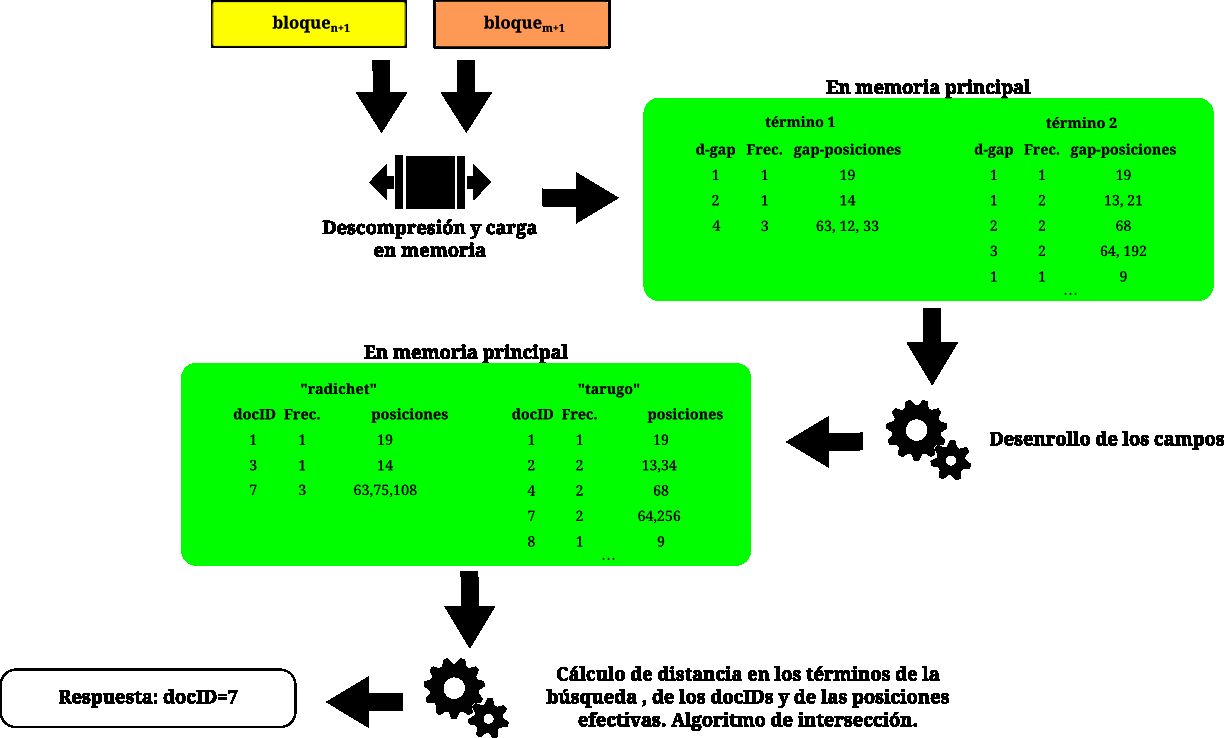
\includegraphics[scale=0.8]{./Images/consulta2.png}
\caption{Obtención de las posiciones a partir de la descompresion de bloques}
\label{fig:consulta2}
\end{figure}


\subsubsection{Algoritmo de intersección}

La consulta de frases implica que la consulta es de tipo booleana, por lo que se la puede ver de la siguiente forma: 
\[ <<radichet>> AND <<tarugo>> \]
Los documentos entregados como resultado de esta consulta serán:
\begin{enumerate}
	\item los que contengan ambos términos y
	\item los que tengan a <<radichet>> en la posición \textit{i} y a <<tarugo>> en \textit{i+1}.
\end{enumerate}

Para resolver el primer punto se utiliza la frecuencia absoluta de los términos (que es la cantidad de documentos en los que aparece cada uno). En el ejemplo, el término <<radichet>> tiene frecuencia 3 y <<tarugo>> 23 por lo que, la máxima cantidad de documentos que podrán cumplir con los requisitos, serán 3. 
Finalmente se ve que solo 2 documentos (el 1 y el 7) contienen a ambos términos).

El segundo punto se resuelve recorriendo la lista de posiciones de los documentos 1 y 7 para cada término en simultaneo.

Finalmente, los documentos que cumplen con los dos puntos son presentados como resultado. En el ejemplo solo el documento de docID $=$ 7 cumple con los requisitos (<<radichet>> en posición 63 y <<tarugo>> en 64).





\section{XR: experimental}

\subsection{Corrector ortográfico}

La idea detrás de un corrector ortográfico es poder darle al usuario respuestas a sus consultas que pueden ser igual o más relevantes que lo que él buscó inicialmente. 

%Para ello se tomar como referencia a \cite{norvigSP}.

Lo que haríamos, aprovechando que tenemos el Diccionario y sus frecuencias absolutas en memoria principal, es hacer las comparaciones utilizando las distancias de edición o de Levenshtein, [\textit{ver \citet[p.~58]{Manning:2008}(\citeyear{Manning:2008})}], para cada palabra de la frase buscada y retornar una frase (o varias) con las más frecuentes, para darla como opción de búsqueda.

Utilizaremos para ello el algoritmo de \citeauthor{norvigSP}, el cual tiene el balance perfecto entre eficiencia y sencillez.



\bibliography{Referencias}

\end{document}
